% 
% Background
% 

% DCN: This subsection is short. Let's move it to the discussion of the 
% benefits of modeling, near the end of the chapter.
%
% \subsection{Previous Computational Models of Autism}
% 
% The formal and explicit nature of computational cognitive modeling suggests a novel approach to autism research.  In order for computational models to be useful in this endeavor, they must be constrained by both bottom-up (neurobiological mechanisms) and by top-down (observed behavior) considerations.  It is not at all clear that the current computational models attempting to provide explanations for the behavior of people with autism have accomplished these goals.  Previous computational models have been published attempting to address various behavioral aspects of autism including poor generalizing~\cite{CohenIL:1994:AutismLearning,GustafssonL:1997:AutismMaps}, Weak Central Coherence~\cite{OLoughlinC:2000:Coherence}, overselectivity~\cite{McClellandJL:2000:Autism}, as well as Grossberg \& Seidman (2006)~\nocite{RefWorks:146} ambitious computational framework seeking to explain multiple aspects of autism including poor generalization as well as cognitive and emotional issues.

% A short coming of many of the existing models of autism is their fairly abstract in nature, making little contact with specific neurobiological considerations~\cite{CohenIL:1994:AutismLearning,McClellandJL:2000:Autism,OLoughlinC:2000:Coherence}.  Even those models of autism which have incorporated biology into their framework have thus far only matched qualitative patterns of behavior in people with ASD, not attempting to account for any quantitative behavioral data~\cite{GustafssonL:1997:AutismMaps,RefWorks:146}.  Models more tightly coupled with observed functional properties of neurobiological systems and constrained by actual behavioral data will be able to more precisely inform theories of ASD. 

\subsection{Dopamine \& Temporal Difference Learning}
Our account of the role of the midbrain DA system in autistic behavior builds on findings and theories concerning the role played by DA in learning, as well as its relationship to PFC. Analyzing the response profile of DA neurons in the basal ganglia of monkeys, Schultz et al. (1997)~\nocite{schultz97td} demonstrated that DA cells appear to encode a prediction error in the amount of future reward to be delivered during the performance of a task. In other words, these cells seem to encode a \emph{change in expected future reward}. This is interesting because a measure of change in expected future reward is a key variable in a powerful reinforcement learning algorithm known as Temporal Difference (TD) learning. In TD learning, the change in expected future reward is know as the TD Error. Across two consecutive time steps the TD Error is given by: 
\begin{equation}\delta(t) = r(t) + \gamma V(t+1) - V(t)\end{equation}

Where $r(t)$ is a reward value that is delivered, at each time step, based on performance (e.g., $r(t) = 1$ for correct performance and $r(t)=0$ on time steps when no reward is presented), $V(t)$ and $V(t+1)$ are the expected future rewards at times $t$ and $t+1$ respectively, \begin{math}\delta(t)\end{math} is the TD Error, and \begin{math}\gamma\end{math} is a constant discounting factor, where \begin{math}0 < \gamma \leq 1\end{math}. Adjusting \begin{math}\gamma\end{math} changes the amount by which temporally distant rewards are discounted as compared to rewards that can be obtained sooner.

This formal connection has led researchers to characterize the role of DA neurons in the brain's learning mechanisms~\cite{BartoAG:1994:TDLearning,MontaguePR:1996:Dopamine}, equating the firing rate of the DA cells with the amount of change in expected future reward, or TD Error. Neurally plausible implementations of TD learning have been implemented and have been used to model the learning of motor sequences in the striatum~\cite{MontaguePR:1996:Dopamine}, driven by the reward-prediction DA signal. Reinforcement learning models of this kind have been highly successful at accounting for a broad range of both behavioral and neuroscientific data~\cite{DayanP:2008:Ugly}.


%\begin{figure}
% 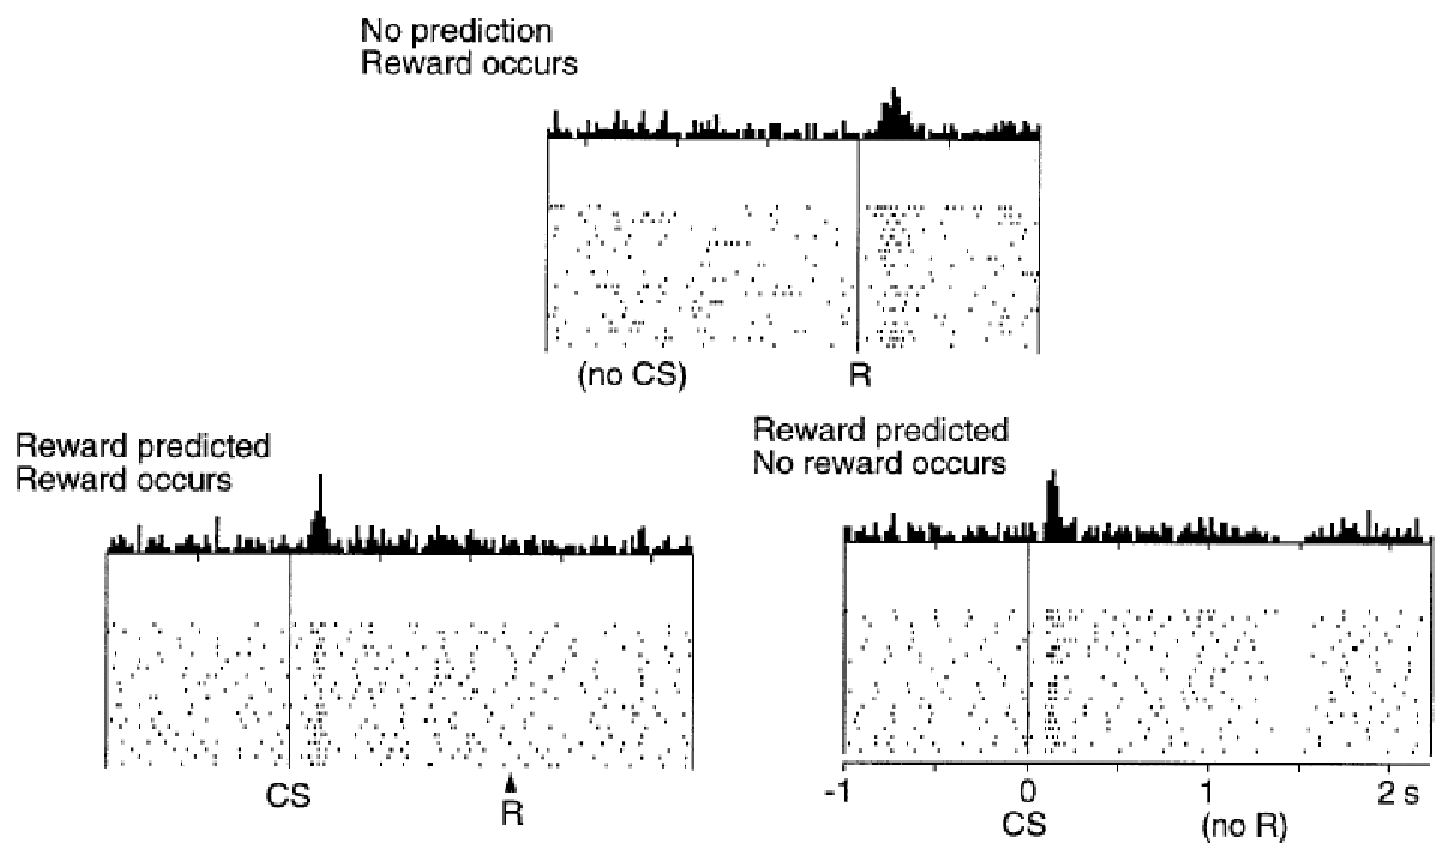
\includegraphics[width=15cm]{figures/schultz}
% \caption{Firing rates of midbrain dopamine neurons of the basal ganglia during classical conditioning (Adapted from Schultz et al., 1997)}
% \label{schultz}
%\end{figure}


% \bigskip

\subsection{Computational Models of Prefrontal Cortex}
The modeling work presented in this chapter is built upon an established computational framework for understanding interactions between PFC and the DA system during tasks requiring cognitive control and cognitive flexibility. One of the primary insights of this framework is that the DA based TD learning mechanism might be used to learn, from experience, when to robustly maintain current representations in the PFC versus allowing updating to occur~\cite{BraverTS:2000:Control}. As described earlier, it is helpful to think of the maintenance versus updating of PFC in terms of a gating mechanism. The key insight is that, in addition to driving the learning of \emph{overt} motor sequences, the TD Error, encoded in the firing rate of DA cells, can be used to learn \emph{covert} actions, such as when to open and when to shut the gate on PFC representations. By building computational models of PFC function using this framework, researchers have shown that this account is plausible~\cite{BraverTS:2000:Control,OReillyRC:2002:IDED}. In these models, PFC control representations are actively maintained in the sustained firing patterns of the modeled PFC pyramidal cells. For example, the PFC can encode, and actively maintain, a representation of ``pay attention to the color of the stimuli''. This maintained pattern of activity can then provide a ``top-down'' bias, up-modulating pathways in posterior brain areas associated with the processing of stimulus color~\cite{CohenJD:1990:Stroop}. The biasing provided by PFC can be used to drive weaker, less automatic, behaviors (e.g., naming the ink color as opposed to reading the word in the Stroop task~\cite{StroopJR:1935:Interference}), as appropriate. This activation based modulation is thought to support our ability to provide cognitive control over behavior~\cite{CohenJD:1992:Schizophrenia,MillerEK:2001:PFC}. The DA based adaptive gating mechanism can signal to PFC when it is appropriate to strengthen the maintenance of the representation currently encoded (i.e., close the gate). This occurs when a positive TD Error arises, signifying a positive change in expected future reward. In other words, when we are doing better than expected, close the gate on PFC representations, so we are more likely to keep doing the same thing. Conversely, if we start to perform worse than expected, possibly due to task contingencies changing, resulting in a negative TD Error (i.e., DA cells firing below their base rate), this signals that we are not performing as well as expected. The negative TD error can be used as a gating signal on PFC representations, causing the gate to open, allowing a new control representation to replace the old, thereby allowing for the flexible adjustment of controlled behavior.

Along with providing a neural mechanism that can learn to appropriately and adaptively gate PFC representations, these models have also been successful at relating frontal disturbances, such as those found in schizophrenia, to deficits in cognitive control~\cite{CohenJD:1992:Schizophrenia} and cognitive flexibility~\cite{BraverTS:1999:Schizophrenia,OReillyRC:2002:IDED}. One computational model that included this form of PFC/DA interaction, called \emph{XT}~\cite{RougierNP:2005:XT}, was the first neuroscientific model able to provide quantitative fits to a hallmark task of cognitive control, the Stroop task~\cite{StroopJR:1935:Interference}, and a widely used measure of cognitive flexibility, the Wisconsin Card Sort Task (WCST)~\cite{BergEA:1948:WCST}, in both neurologically intact and frontally damaged people. In the next chapter, we explain how we used the XT model to investigate whether a dysfunctional DA based gating mechansim can capture the specific executive profile of people with autism.
